\documentclass[a4paper,10pt]{article}

\usepackage[ansinew]{inputenc}
\usepackage[spanish]{babel}
\usepackage{graphicx}
\usepackage{listings}
\usepackage{appendix}
\usepackage{pdfpages}
\usepackage{fancyhdr}
\pagestyle{fancy}

\begin{document}

\lhead{\fancyplain{}{Organizaci\'on de computadoras 66.20 - Turno Martes}}
\rhead{\fancyplain{}{Trabajo Pr\'actico 0}}

\setcounter{page}{2}

\newpage
\thispagestyle{empty}
\tableofcontents

\newpage
\section{Introducci\'on}

En el presente trabajo pr\'actico se busc\'o familiarizarse con las
herramientas de software que se usar\'an en los siguientes trabajos
pr\'acticos. Estas herramientas son el programa GXemul para simular el
entorno de desarrollo y una m\'aquina MIPS corriendo una versi\'on del
sistema operativo NetBSD. Para ello, se escribieron dos programas en
lenguaje C que permiten convertir archivos de texto desde y hacia
plataformas UNIX. 

\section{Resoluci\'on del problema}
Para la resoluci\'on del ejercicio se realiz\'o una funci\'on llamada
``parser'' encargada de la conversi\'on de archivos de textos desde y hacia 
plataformas UNIX. Para poder lograr la conversi\'on se tuvieron que cambiar los caracteres
\textbackslash n por \textbackslash r\textbackslash n para convertir el formato de archivo de UNIX a DOS y la conversi\'on 
inversa para pasar de DOS a UNIX. 

  \subsection{Funcion ``main''}
  En ambos programas se llama a la funci\'on ``parser'' detallada a continuaci\'on, y se retorna el valor de 
  retorno de la misma. Lo \'unico que los diferencia es que en ``unix2dos'' el valor de ``finLinea'' toma el 
  valor de \textbackslash n y finLineaNuevo \textbackslash r\textbackslash n, y en ``dos2unix'' se 
  intercambian esos valores.

  \subsection{Funcion ``parser''}
  Esta funci\'on se encarga de obtener las opciones de ejecuci\'on del programa utilizando la funcion ``getopt'' y, en base
  a eso, llamar a la funci\'on ``traducirFormato'', pasandole los parametros correspondientes.
  \newline
  Para la captura de los par\'ametros opcionales que pueden utilizarse al 
  llamar el programa se decidi\'o utilizar la funci\'on:
  \newline
  {\bf getopt(int argc,char\*\* argv,char\* options)}. 
  \newline
  Esta decisi\'on se tomo con el fin de simplificar el c\'odigo necesario para la resoluci\'on del parseo de los
  argumentos; dado que, de este modo, se evita generar c\'odigo que tenga
  en cuenta todas las combinaciones posibles de los mismos. As\'i como
  tambi\'en, para que pueda ser extensible; es decir, pueda expandirse
  f\'acilmente el programa en caso de desear agregar par\'ametros para
  ejecutar el mismo.
  El cuerpo de la funcion 'main' consiste de:
  \begin{itemize}
  \item Se utiliza {\bf getopt} para obtener los par\'ametros con los que se invoca el programa. Y se 
    utilizan flags para determinar en que situaci\'on de las posibles se encuentra.
  \item Se abren los archivos origen, en modo lectura, y destino, en modo escritura escritura (de esta
    forma se crea el archivo, si no existe), en los casos en los que sea necesario. Dado que si la funci\'on
    se invoca en alguna de las posibles combinaciones que permiten stdin y/o stdout, se utiliza dichos 
    archivos.
  \item Se llama a la funcion {\bf traducirFormato}, detallada previamente, con los par\'ametros 
    correspondientes al modo del que fue invocada la aplicaci\'on.
  \item Se cierran ambos archivos, en caso de que corresponda.
  \end{itemize}


  \subsection{Funci\'on ``traducirFormato''}
  Para parsear el archivo de entrada se fue obteniendo caracter a caracter y
  se fue comparando de que no se tratara del fin de linea
  correspondiente a la plataforma del archivo de entrada, de
  encontrarnos en esa situaci\'on se escribe el caracter al archivo de
  salida. Si nos encontramos en el caso de fin de linea se escribe en el
  archivo de salida el fin de linea de la otra plataforma. 
  El encabezado de la funci\'on es el siguiente:
  \newline
  {\bf void parser(FILE * origen, FILE * destino, char *finLinea, char *finLineaNuevo)}
  \newline
  Los par\'ametros que recibe son:

  \begin{itemize}
  \item {\bf FILE *origen:}
    Descriptor del archivo origen. Debe existir y estar abierto correctamente.
  \item {\bf FILE *destino:}
    Descriptor del archivo destino, en el que se almacenara el archivo resultante. Debe estar abierto correctamente.
  \item {\bf char *finLinea:}
    Cadena que almacena la cadena de fin de linea del archivo origen.
  \item {\bf char *finLineaNuevo:}
    Cadena que almacena la cadena de fin de linea del archivo destino.
  \end{itemize}

\section{Preparando el ambiente para NetBSD}
  Para probar el trabajo pr\'actico, lo primero que se debe realizar es enviar el c\'odigo fuente al entorno
  del NetBSD. Se considera que el NetBSD se encuentra corriendo y que se ha creado el loopback necesario. Para ello, se deben realizar los siguientes pasos:
  \begin{enumerate}
   \item Abrir una consola e ingresar en modo root.
   \item Copiar la carpeta ``Codigo`` del cd, a la carpeta del usuario gxemul:
    \newline 
      {\bf hostOS\# cp -r \textbackslash Unidad\_de\_CD\textbackslash Codigo \textbackslash home\textbackslash gxemul}
   \item Conectar con el NetBSD a trav\'es de un t\'unel, se debe ingresar el password correspondiente al 
	 usuario root del NetBSD:
    \newline
      {\bf hostOS\# ssh -p 2222 root@127.0.0.1}
   \item Crear una carpeta para el Tp0, opcional se utiliza para una mejor organizaci\'on:
    \newline 
    {\bf guestOS\# mkdir Tp0}
   \item Copiar la carpeta ''Codigo`` a la carpeta Tp0 del NetBSD, se debe ingresar el password correspondiente al
         usuario gxemul del sistema operativo host:
   \newline
    {\bf guestOS\# scp -r gxemul@172.20.0.1:\textbackslash home\textbackslash gxemul\textbackslash Codigo \newline Tp0\textbackslash }
  \end{enumerate}

\section{Compilaci\'on en NetBSD}
  \subsection{Generando c\'odigo binario}
    Para poder compilar desde NetBSD y obtener el c\'odigo binario, se debe ejecutar:
    \newline
    {\bf guestOS\# gcc -o unix2dos unix2dos.c} \newline
    {\bf guestOS\# gcc -o dos2unix dos2unix.c}
    \newline
    En ambos casos, se decidi\'o utilizar como nombre archivo de salida (opci\'on -o) el mismo del archivo 
    del c\'odigo fuente.
    
  \subsection{Generando c\'odigo assembly}
    Para poder compilar desde NetBSD y obtener el c\'odigo MIPS generado por el compilador, se debe ejecutar:
    \newline
    {\bf guestOS\# gcc -Wall -O0 -S -mrnames unix2dos.c} 
    \newline
    {\bf guestOS\# gcc -Wall -O0 -S -mrnames dos2unix.c}
    \newline
    Donde:
    \begin{itemize}
      \item {\bf-S:} detiene al compilador luego de generar el assembly.
      \item {\bf-mrnames} (solo para MIPS): indica al compilador que genere la salida utilizando nombre de 
	registro en lugar de n\'umero de registro.
      \item {\bf-O0:} No aplica optimizaciones.
    \end{itemize}
    A continuaci\'on el c\'odigo assembly:
    \subsubsection{unix2dos}
      \lstset{numbers=left, frame=single, breaklines=true}
      \lstinputlisting{../Codigo/dos2unix.s}
    \subsubsection{dos2unix}
      \lstset{numbers=left, frame=single, breaklines=true}
      \lstinputlisting{../Codigo/unix2dos.s}

\section{Ejecutando los programas en NetBSD}
  Para ejecutar el programa, el comando a utilizar es:
  \newline
  {\bf./[nombre de ejecutable] -i [ruta de archivo origen] -o [ruta de archivo destino]}
  \newline
  En caso de que no se utilicen las opciones {\bf ``-i''} (archivo de entrada) y {\bf ``-o''} (archivo de salida) el 
  programa utiliza la entrada estandar (stdin) y salida estandar (stdout). Para ver ejemplos, observar 
  secci\'on de casos de prueba.


\section{Casos de prueba}
En la siguiente secci\'on se detallaran los distintos archivos utilizados para probar el funcionamiento del
programa. Para ello se adjuntaran imagenes de corridas de los mismos; en donde se ense\~{n}a el dump del 
archivo origen, en formato ASCII con barra invertidas para los caracteres de escape, y luego el del 
archivo destino.

  \subsection{Distintas formas de invocaci\'on}
    \subsubsection{Prueba 1}
    Invocaci\'on del programa con par\'ametros -i y -o definidos:
    \begin{itemize}
      \item \textbf{dos2unix}
      \newline	
      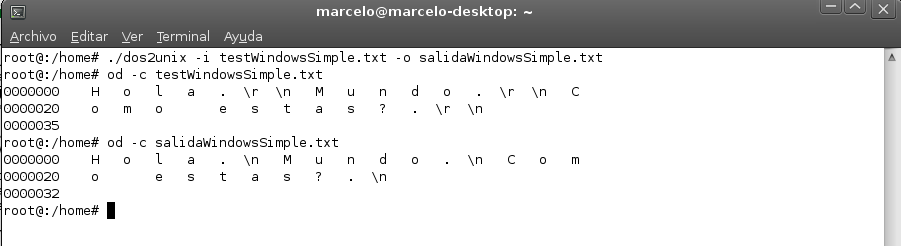
\includegraphics[width=10cm, viewport=0 0 901 246]{../Informe/Imagenes/prueba1-invocacion-dos2unix.png}
      \newline
      En la figura se muestra el contenido de los archivos de entrada y salida. Como es de esperarse, la unica diferencia
      se encuentra en los caracteres de fin de linea, `\textbackslash r\textbackslash n' en el de entrada, y `\textbackslash n' en el de salida.
      \item \textbf{unix2dos}
      \newline
      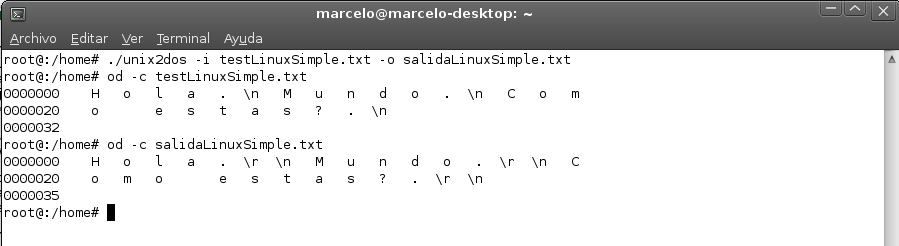
\includegraphics[width=10cm, viewport=0 0 899 246]{../Informe/Imagenes/prueba1-invocacion-unix2dos.png}
      \newline
      En este caso, el pasaje es inverso al anterior: se pasa de `\textbackslash n' a `\textbackslash r\textbackslash n'.	
      \newline
      Nota: En las siguientes pruebas de esta secci\'on se omitira mostrar el contenido del archivo de entrada, ya que es el mismo
      para las siguientes pruebas. En secciones posteriores se utilizar\'an distintos archivos.
    \end{itemize}

    \subsubsection{Prueba 2}
    Invocaci\'on del programa con par\'ametros -i definido (se utiliza un archivo de entrada y se muestra
    la salida por salida est\'andar):
    \begin{itemize}
      \item \textbf{dos2unix}
      \newline
      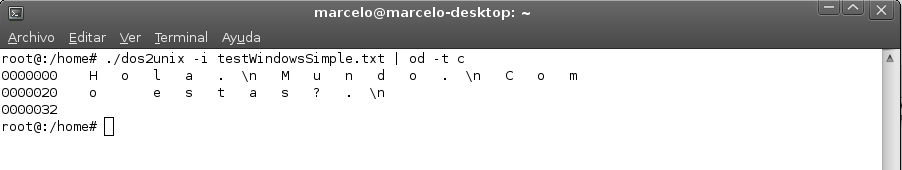
\includegraphics[width=10cm, viewport=0 0 902 170]{../Informe/Imagenes/prueba2-invocacion-dos2unix.png}
      \newline	
      En la figura puede verse como al no utilizar la opci\'on `-o' se muestra el archivo de salida por
      salida est\'andar de manera correcta.	
      \item \textbf{unix2dos}
      \newline 
      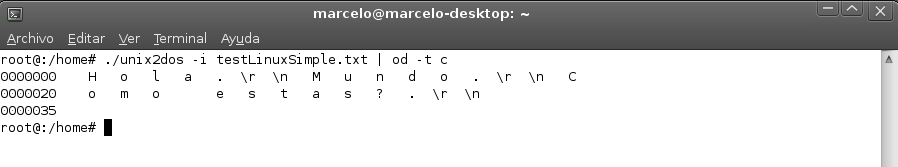
\includegraphics[width=10cm, viewport=0 0 898 167]{../Informe/Imagenes/prueba2-invocacion-unix2dos.png}		
      \newline
      Como en el caso `dos2unix', se muestra el archivo de salida por salida est\'andar.
    \end{itemize}

    \subsubsection{Prueba 3}
    Invocaci\'on del programa con par\'ametros -i igual a ``-'' (flujo est\'andar stdin):
      \begin{itemize}
      \item \textbf{dos2unix}
      \newline 
      %\ falta
      %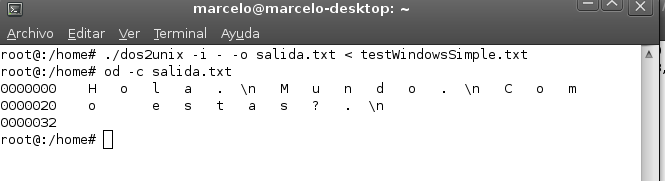
\includegraphics[width=10cm, bb=0 0 901 246]{../Informe/Imagenes/prueba3-invocacion-dos2unix.png}
      %\newline	
      En este caso, se explicita el uso de la entrada est\'andar. La salida es almacenada en un archivo
      de salida. 
      \item \textbf{unix2dos}
      \newline 
      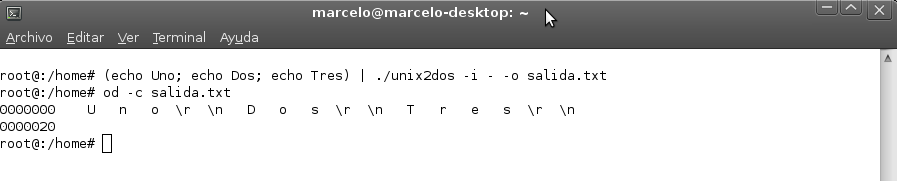
\includegraphics[width=10cm, viewport=0 0 897 181]{../Informe/Imagenes/prueba3-invocacion-unix2dos.png}	
      \newline
      Como en el caso, `dos2unix', se explicita el uso de la entrada est\'andar, almacenando la salida en un archivo espec\'ificado por par\'ametro.
      Se muestra el resultado obtenido en el archivo de salida, utilizando od.
      \textcolor{red}{COMENTAR}
    \end{itemize}

    \subsubsection{Prueba 4}
    Invocaci\'on del programa con par\'ametros -i definido y -o igual a ``-'' (flujo est\'andar stdout):
      \begin{itemize}
      \item \textbf{dos2unix}
      \newline
      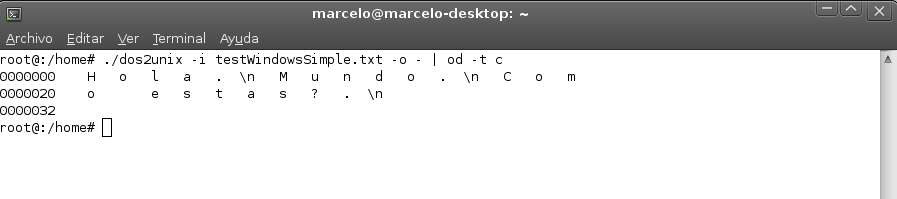
\includegraphics[width=10cm, viewport=0 0 897 199]{../Informe/Imagenes/prueba4-invocacion-dos2unix.png}
      \newline	
      Como se muestra en la figura, se explicita el uso de la salida est\'andar y tomando como entrada un archivo predefinido utilizando como opciones 
      `-i archivoInput -o -'.
      \item \textbf{unix2dos}
      \newline
      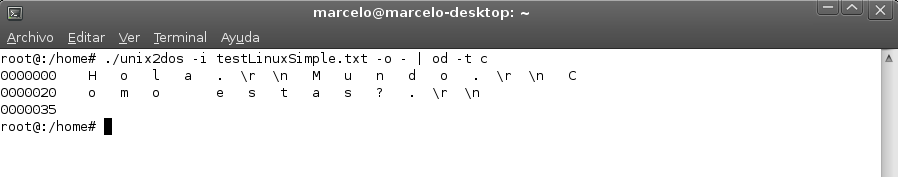
\includegraphics[width=10cm, viewport=0 0 898 177]{../Informe/Imagenes/prueba4-invocacion-unix2dos.png}	
      \newline
      Como en el caso `dos2unix', se explicita el uso de la salida est\'andar tomando como entrada un archivo predefinido e invocando al programa
      utilizando como opciones `-i archivoInput -o -'.
      \textcolor{red}{COMENTAR}
      \end{itemize}

    \subsubsection{Prueba 5}
    Invocaci\'on del programa con -o indefinido:
      \begin{itemize}
      \item \textbf{dos2unix}
      \newline
      %\ falta
      %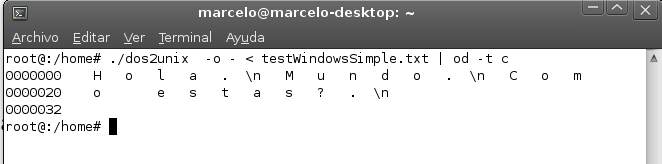
\includegraphics[width=10cm, bb=0 0 901 246]{prueba5-invocacion-dos2unix.png}
      %\newline	
      Como se muestra en la figura, se utiliza la entrada y salida est\'andar. Se invoca al programa con las opciones
      ` -i - -o -'.
      \item \textbf{unix2dos}
      \newline
      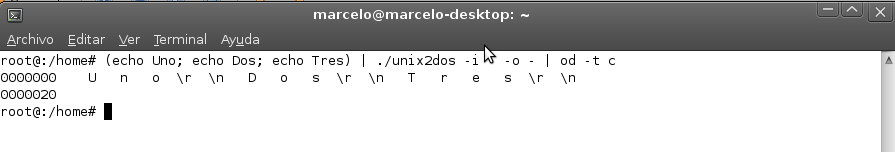
\includegraphics[width=10cm, viewport=0 0 895 152]{../Informe/Imagenes/prueba5-invocacion-unix2dos.png}	
      \newline
      Como en el caso `dos2unix', se utiliza la entrada y la salida est\'andar. Se invoca al programa con las opciones
      ` -i - -o -'.
      \textcolor{red}{COMENTAR}
      \end{itemize}


    \subsubsection{Prueba 6}
    Invocaci\'on del programa con entrada por stdin y salida por stdout:
      \begin{itemize}
      \item \textbf{dos2unix}
      %\newline
      %\ falta
      %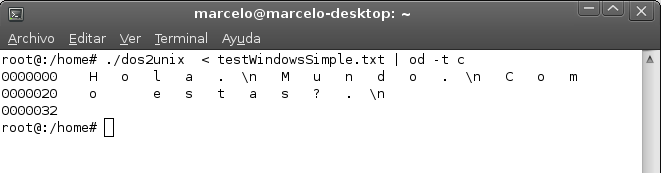
\includegraphics[width=10cm, bb=0 0 901 246]{../Informe/Imagenes/prueba6-invocacion-dos2unix.png}
      \newline
      Como se muestra en la figura, se invoca al programa sin ning\'un par\'ametro y el mismo toma como comportamiento por defecto
      la entrada por entrada est\'andar y la salida por salida est\'andar.
      \item \textbf{unix2dos}
      \newline
      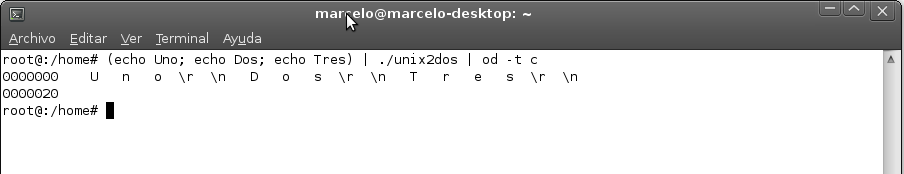
\includegraphics[width=8cm, viewport=0 0 904 174]{../Informe/Imagenes/prueba6-invocacion-unix2dos.png}	      
      \newline
      Como en el caso de `dos2unix', se invoca al programa sin ning\'un par\'ametro y el programa toma su comportamiento
      por defecto.
      \textcolor{red}{COMENTAR}
      \end{itemize}

  \subsection{Distintos archivos de prueba}
    \subsubsection{Prueba 1}
    Utilizaci\'on de un archivo de origen vac\'io:
      \begin{itemize}
      \item \textbf{dos2unix}
      \newline
      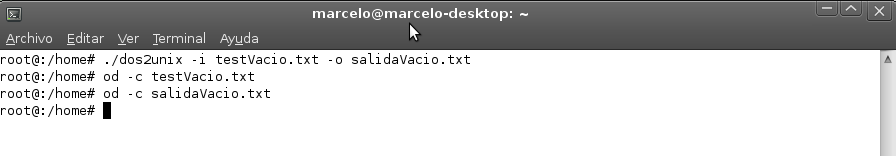
\includegraphics[width=8cm, viewport=0 0 896 156]{../Informe/Imagenes/prueba1-archivo-dos2unix.png}
      \newline	
      Al pasar un archivo vacio como entrada se crea un archivo vacio, como es de esperarse.
      \item \textbf{unix2dos}
      \newline
      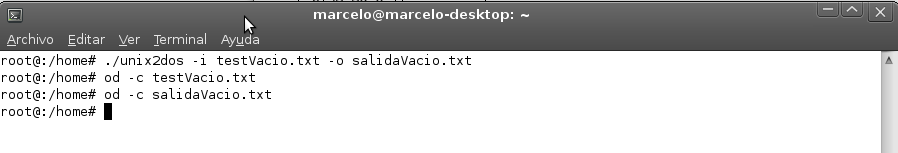
\includegraphics[width=8cm, viewport=0 0 898 153]{../Informe/Imagenes/prueba1-archivo-unix2dos.png}	
      \newline
      \textcolor{red}{COMENTAR}
      \end{itemize}

    \subsubsection{Prueba 2}
    Utilizaci\'on de un archivo inexistente:
      \begin{itemize}
      \item \textbf{dos2unix}
      \newline
      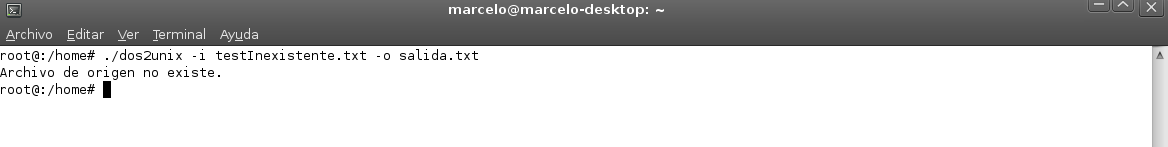
\includegraphics[width=8cm, viewport=0 0 1168 147]{../Informe/Imagenes/prueba2-archivo-dos2unix.png}
      \newline	
      \textcolor{red}{COMENTAR}
      \item \textbf{unix2dos}
      \newline
      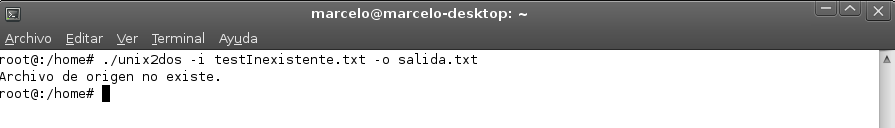
\includegraphics[width=8cm, viewport=0 0 895 128]{../Informe/Imagenes/prueba2-archivo-unix2dos.png}
      \newline
      \textcolor{red}{COMENTAR}
      \end{itemize}

    \subsubsection{Prueba 3}
    Utilizaci\'on de un archivo complejo:
      \begin{itemize}
      \item \textbf{dos2unix}
      \newline
      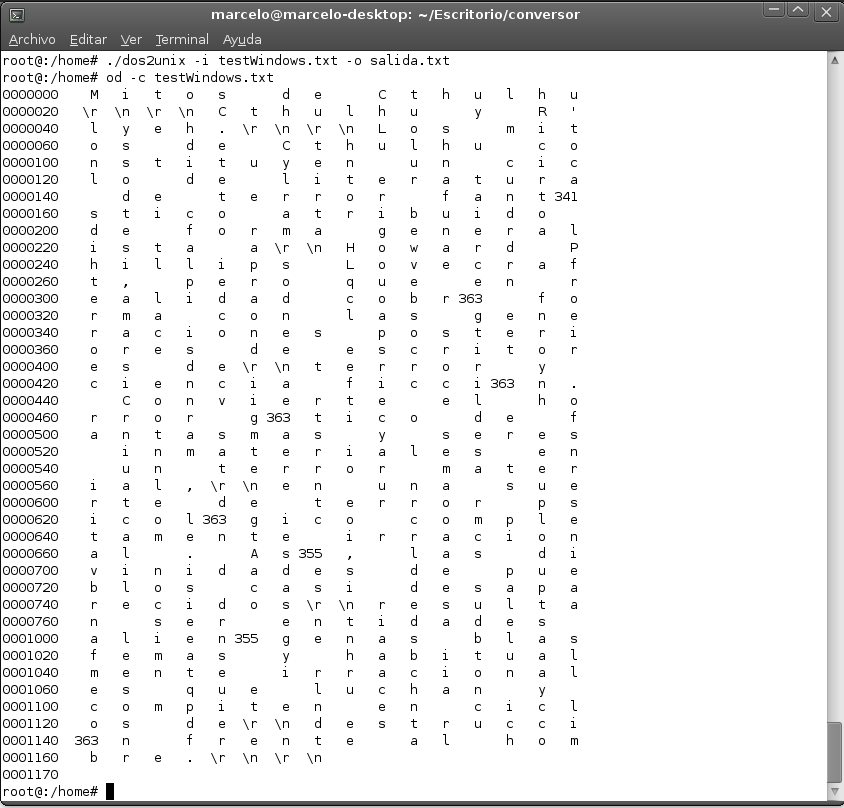
\includegraphics[width=10cm, viewport=0 0 844 808]{../Informe/Imagenes/prueba3-archivo-dos2unix1.png}
      \newline
      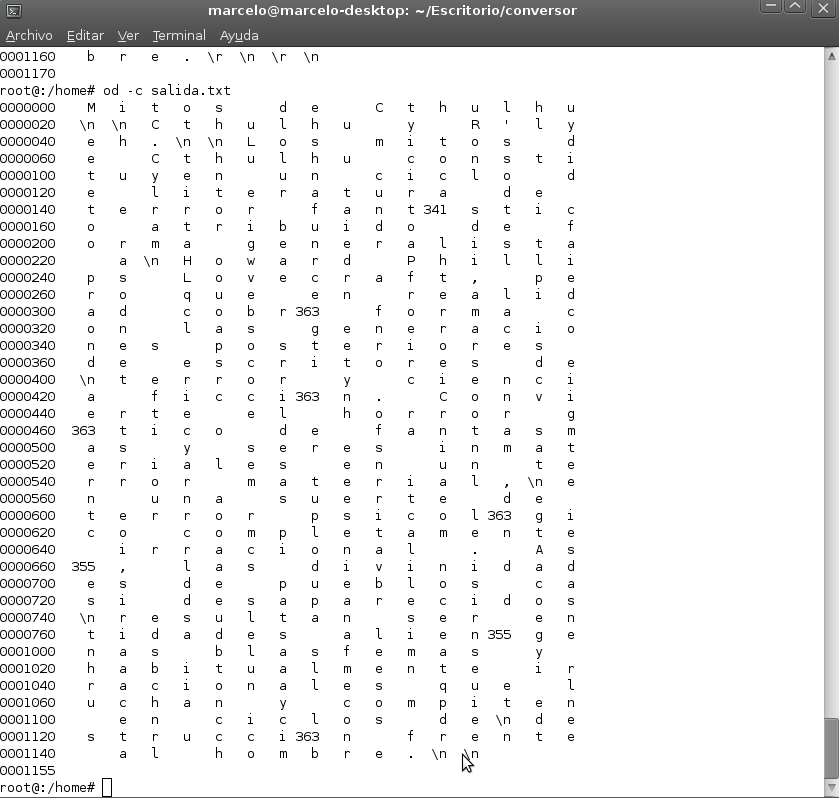
\includegraphics[width=10cm, viewport=0 0 839 798]{../Informe/Imagenes/prueba3-archivo-dos2unix2.png}
      \newline
      \textcolor{red}{COMENTAR}
      \item \textbf{unix2dos}
      \newline
      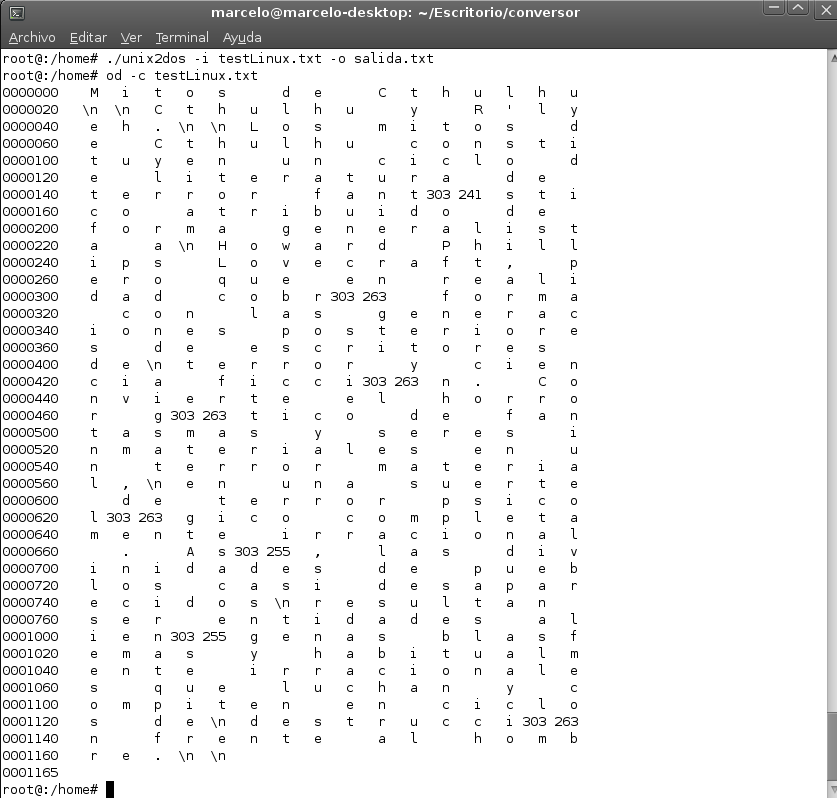
\includegraphics[width=10cm, viewport=0 0 837 798]{../Informe/Imagenes/prueba3-archivo-unix2dos1.png}
      \newline
      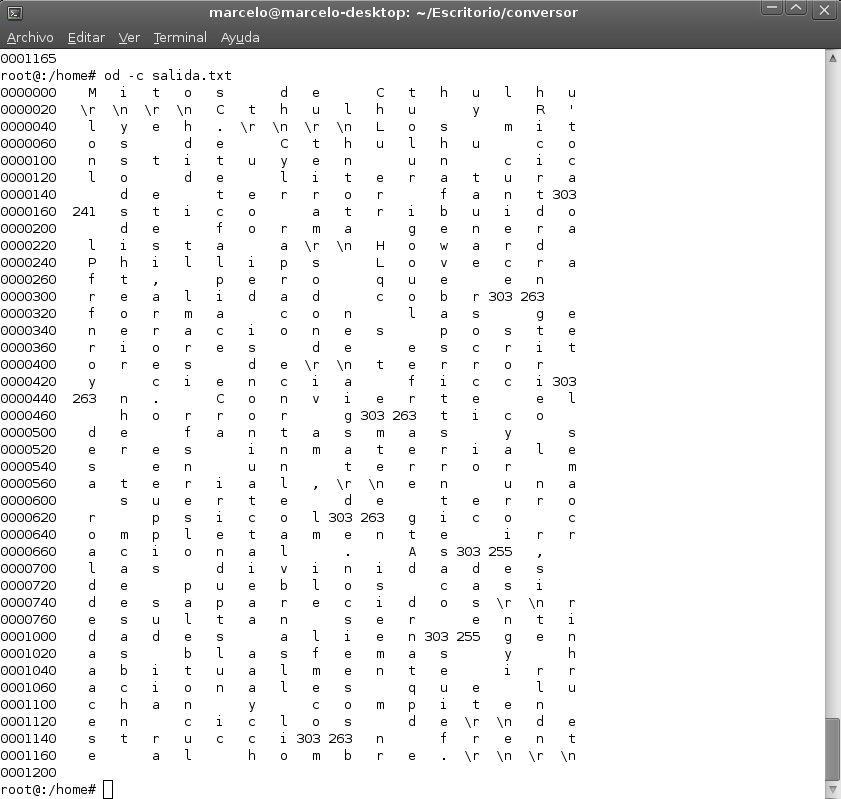
\includegraphics[width=10cm, viewport=0 0 841 799]{../Informe/Imagenes/prueba3-archivo-unix2dos2.png}		
      \newline
      \textcolor{red}{COMENTAR}
      \end{itemize}
    \subsubsection{Prueba 4}
    Conversi\'on de un archivo de un formato al otro, y el resultado convertirlo al formato original:
      \begin{itemize}
      \item \textbf{dos2unix}
      \newline
      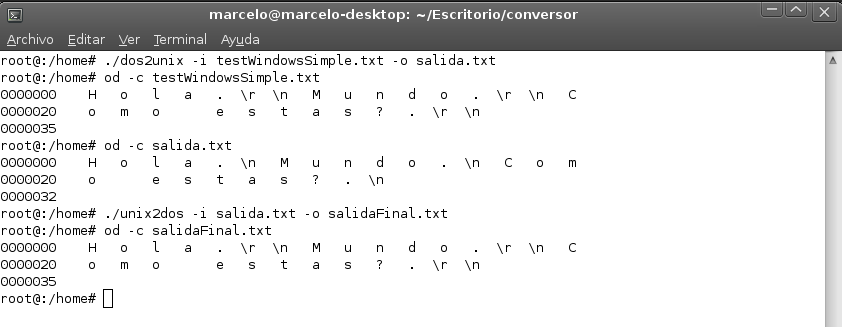
\includegraphics[width=10cm, viewport=0 0 842 328]{../Informe/Imagenes/prueba4-archivo-dos2unix.png}	
      \newline
      \textcolor{red}{COMENTAR}
      \item \textbf{unix2dos}
      \newline
      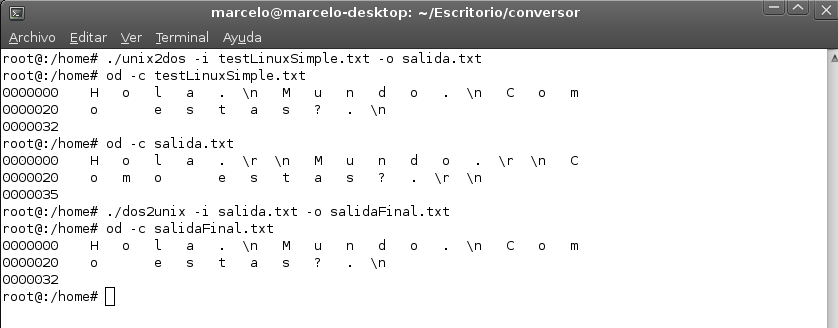
\includegraphics[width=10cm, viewport=0 0 838 328]{../Informe/Imagenes/prueba4-archivo-unix2dos.png}	
      \newline
      \textcolor{red}{COMENTAR}
      \end{itemize}

\section{Conclusiones}
     \textcolor{red}{Completar...}


%APENDICES
\appendix
\newpage
\section{C\'odigo Fuente}
  \subsection{unix2dos.c}
    \lstset{numbers=left, frame=single, breaklines=true}
    \lstinputlisting{../Codigo/unix2dos.c}
  \subsection{dos2unix.c}
    \lstset{numbers=left, frame=single, breaklines=true}
    \lstinputlisting{../Codigo/dos2unix.c}
  \subsection{conversor.c}
    \lstset{numbers=left, frame=single, breaklines=true}
    \lstinputlisting{../Codigo/conversor.c}

\newpage
\section{Enunciado}
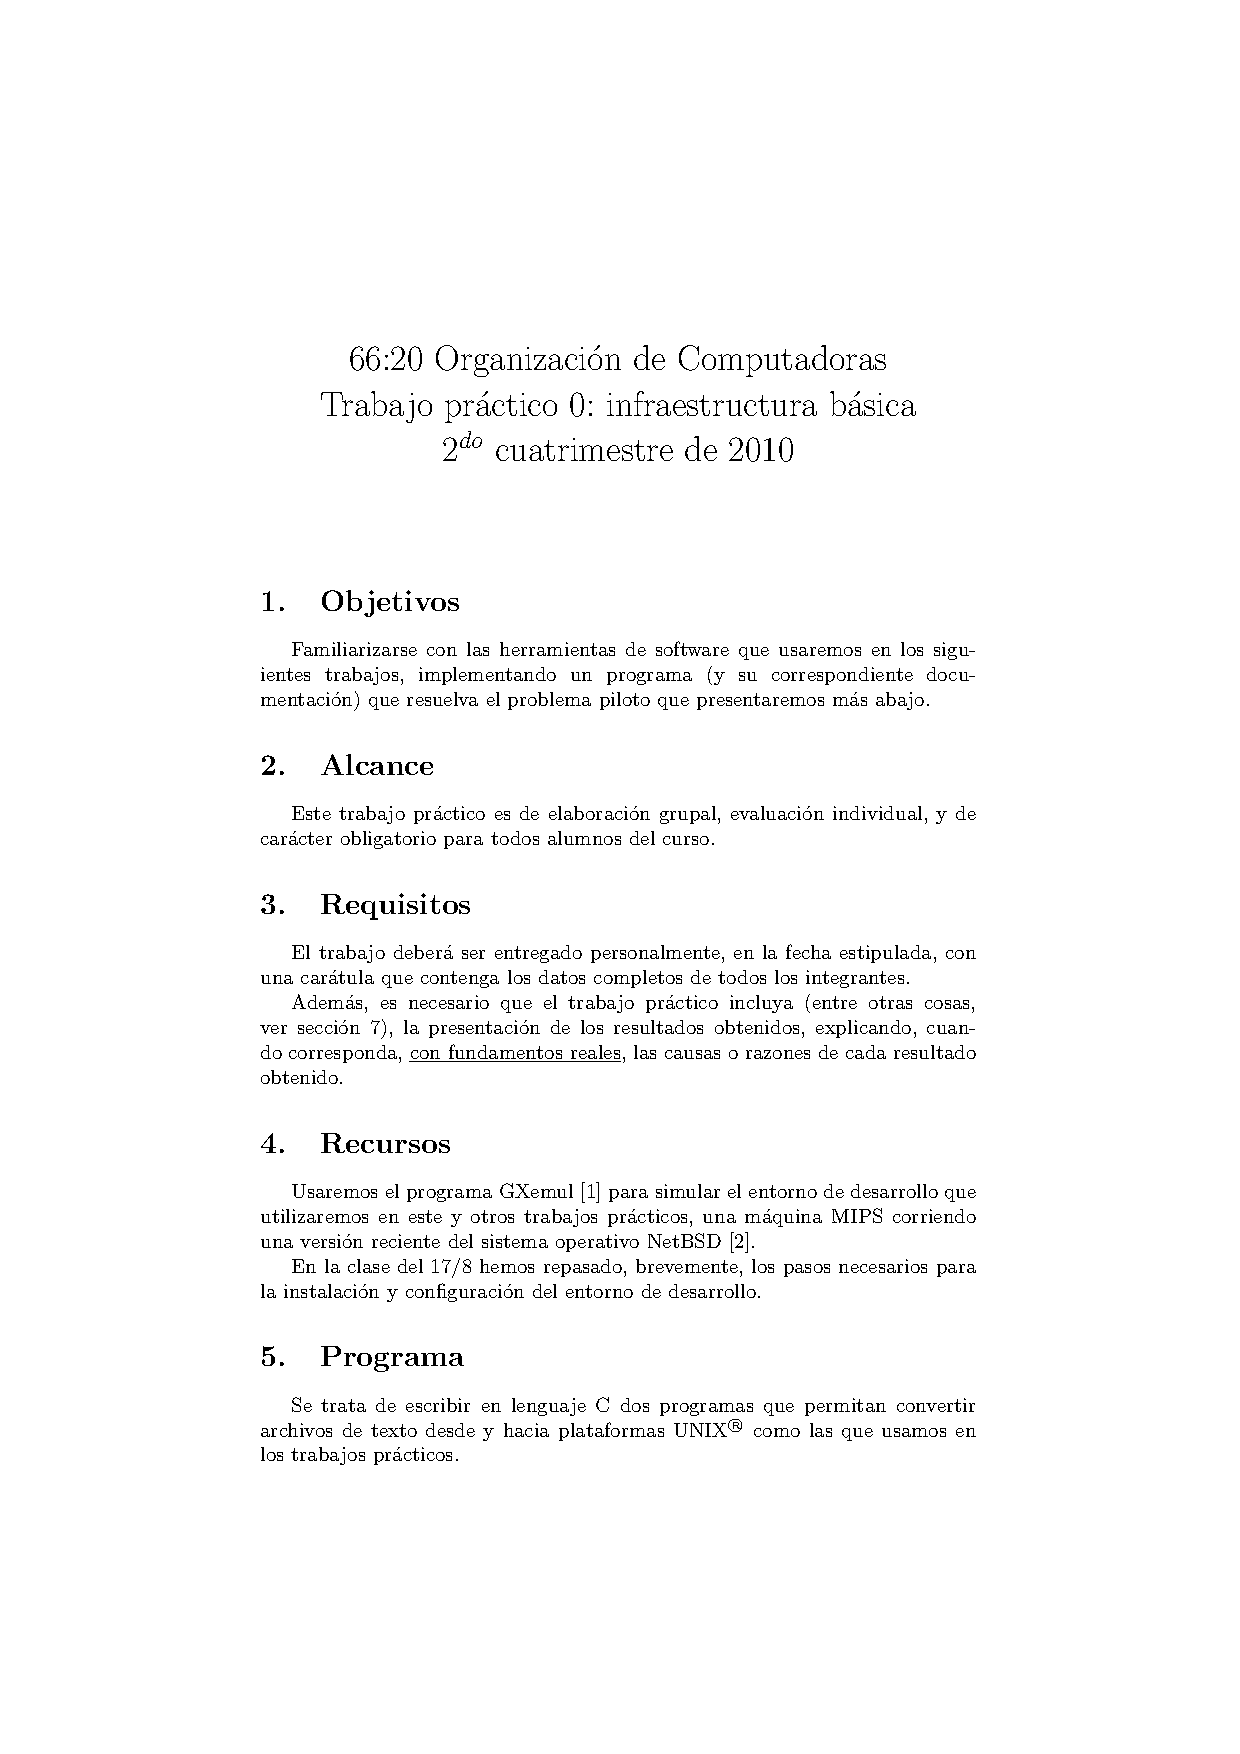
\includepdf[pages=1-3, scale=0.9, pagecommand={\thispagestyle{plain}}]{../tp0-2010-2q.pdf}

\end{document}
